In order to probe the various aspects of the well-established standard model or search for hints of new physics beyond the SM, particle physics experiments preferentially make use of powerful particle accelerators where particles of a certain type are collided in order to probe the constituents of matter and interactions between them. The analyses presented in this thesis are all performed in the context of the CMS experiment located at the Large Hadron Collider (LHC) at CERN near Geneva. \\ 
The first part of this chapter provides an introduction to the LHC. This is followed by an overview of the detector system of the CMS experiment. Afterwards the hitherto periods of collision data taking at the LHC are discussed together with an introduction to the generation of simulated events which are used in the analysis of real data events.  
\section{The Large Hadron Collider}
\label{sec:lhc}
The Large Hadron Collider~\cite{Bruning:782076, 1748-0221-3-08-S08001} is a ring-accelerator designed to provide particle collisions of hadrons. It is built in the tunnel of the former LEP~\cite{LEPdesign} collider 45 -- 170\,m below the ground and has a circumference of 26.7\,km. The LHC is a particle-particle collider and thus composed of two rings with counter-rotating beams. The operation can be performed in different modes with either proton beams or heavy ions like e.g. lead~\footnote{All studies presented in this thesis are based on proton-proton collisions. Thus the operation with heavy ions is not discussed.}. \\
In each beam, protons are grouped together in bunches and accelerated in two evacuated beam pipes using superconducting radio-frequency cavities. With a nominal bunch spacing of 25\,ns the bunch revolution frequency is 40\,MHz. Each of the 2808 individual bunches per beam contains at design conditions $1.15 \times 10^{11}$ protons. In order to bend the beams around the LHC ring superconducting dipole magnets are used with an operation temperature of 1.9\,K. They provide a magnetic field of up to 8.33\,T while additional quadrupole and sextupole magnets are utilized to squeeze and focus the beams.\\  
Before the protons are injected into the LHC they are already pre-accelerated in various smaller accelerators up to a beam energy of 450\,GeV while passing through the injector chain Linac2 -- Proton Synchrotron Booster (PSB) -- Proton Synchrotron (PS) -- Super Proton Synchrotron (SPS). An overview of the accelerator complex at CERN is given in Fig.~\ref{fig:AccComplex}.
\begin{figure}[!tp]
  \centering
  \begin{tabular}{c}
    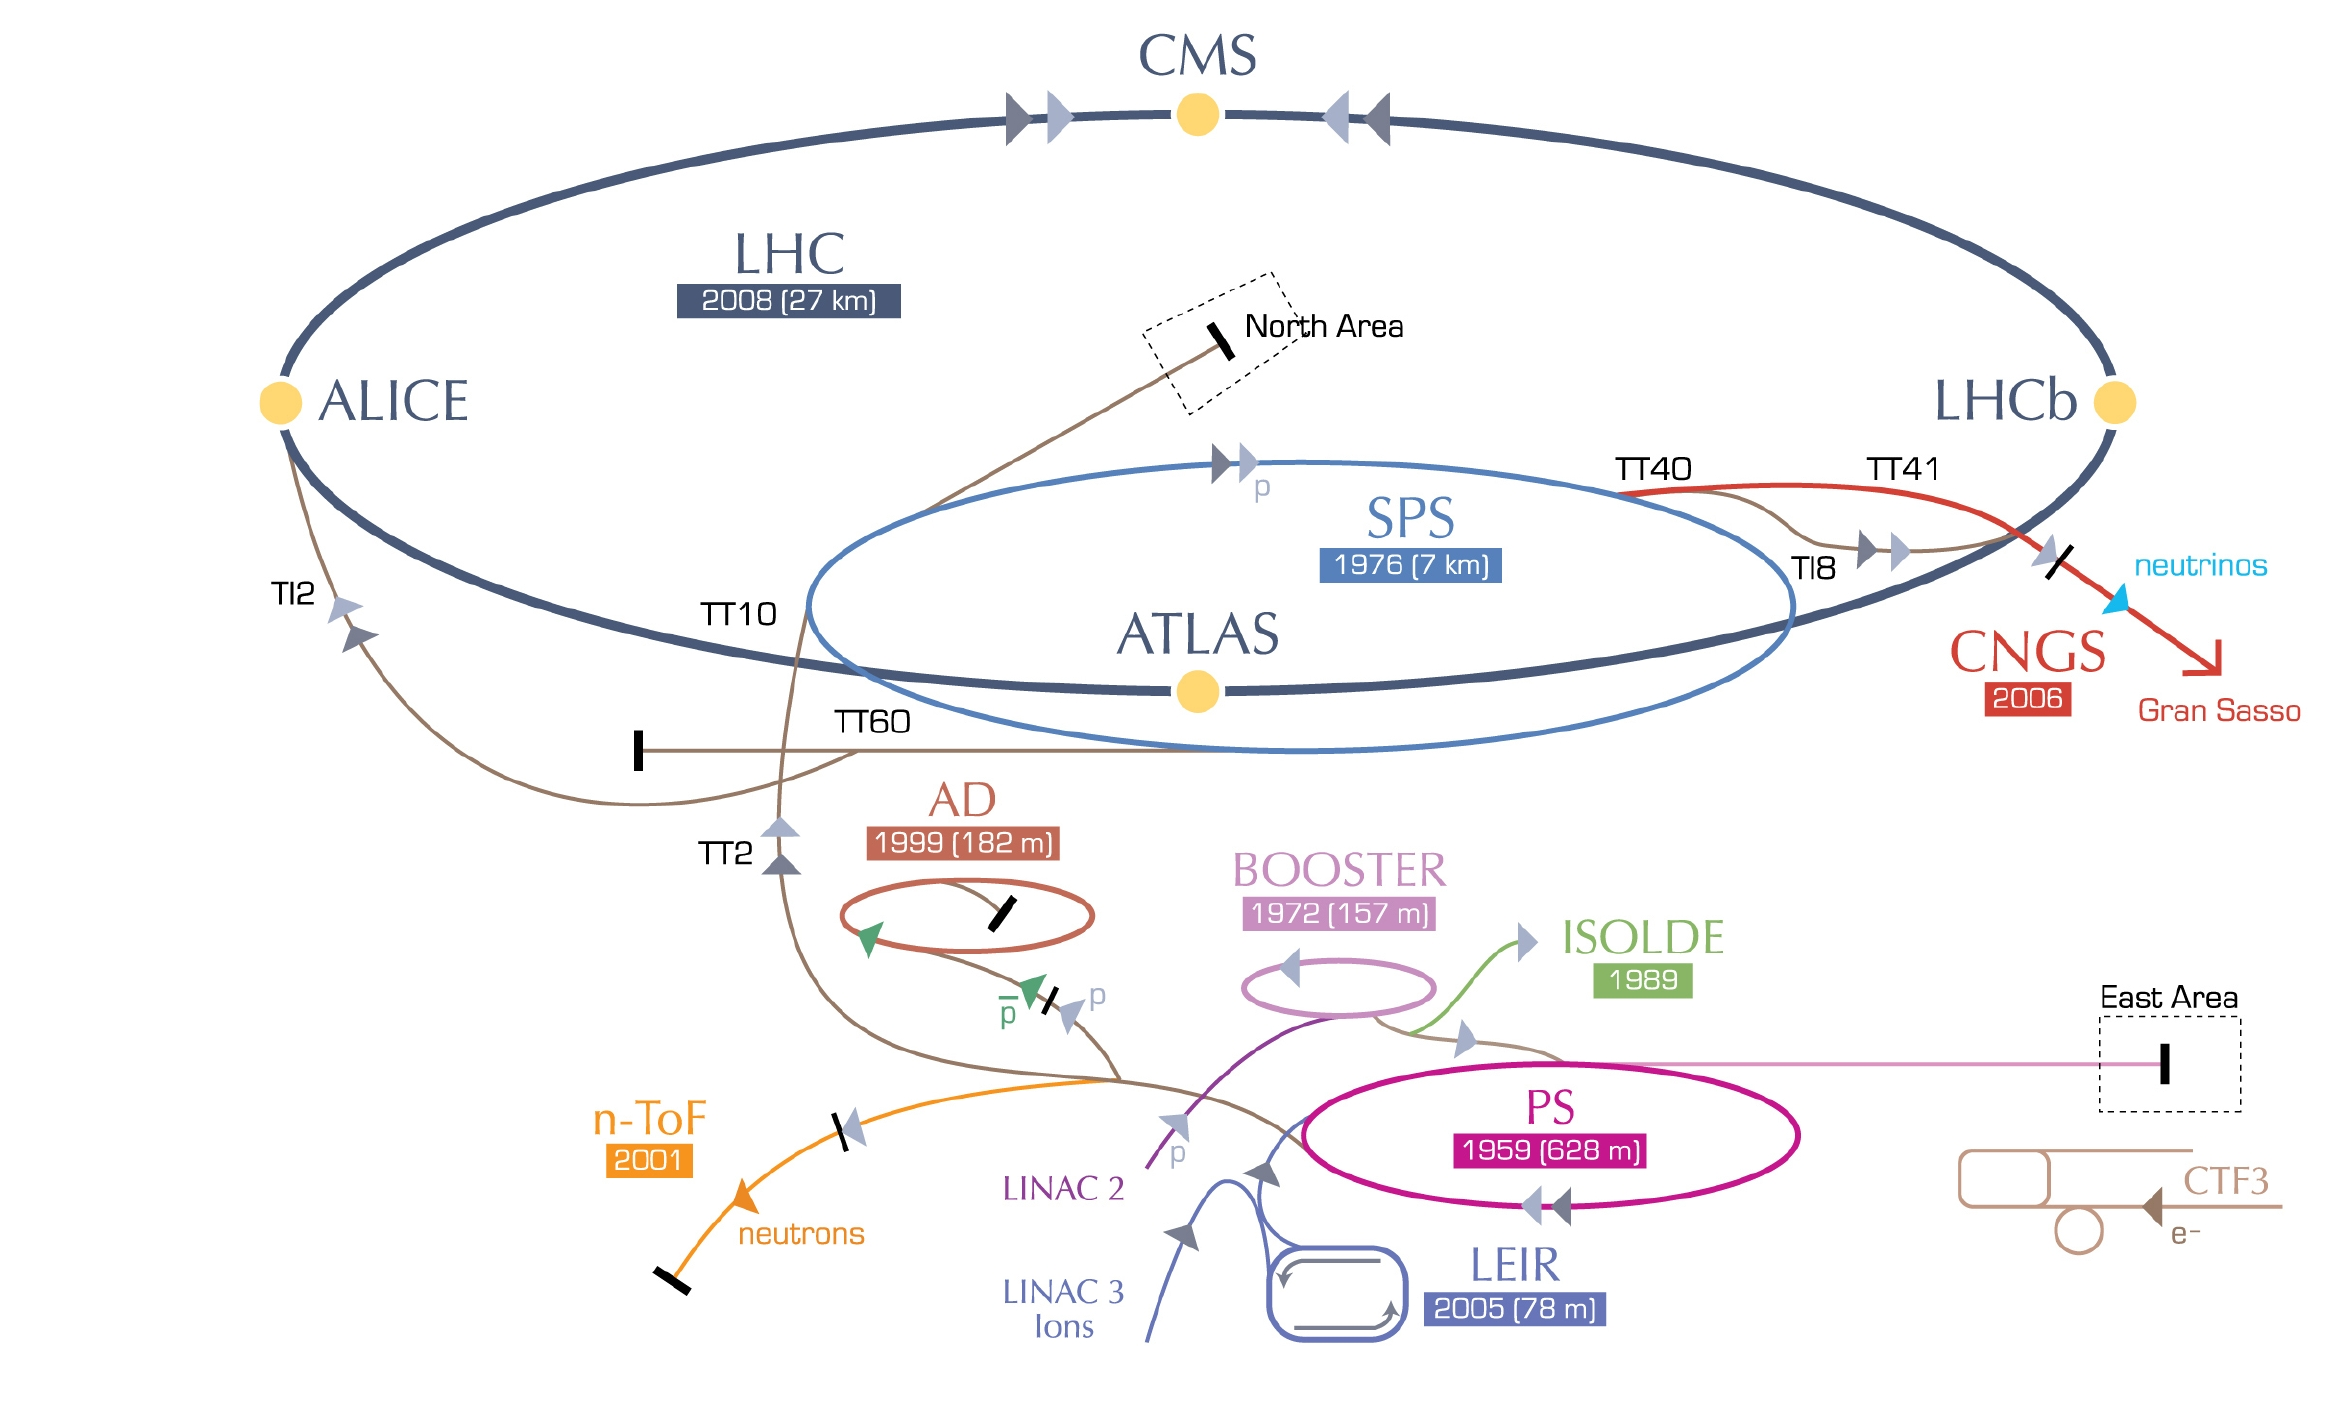
\includegraphics[width=0.8\textwidth]{figures/AcceleratorComplex.jpg}
  \end{tabular}
  \caption{Illustration of the CERN accelerator complex. Numbers below the names of individual machines indicate the year of their first operation. For ring accelerators also the circumference is given. Taken from~\cite{Christiane:1260465}.}
  \label{fig:AccComplex}
\end{figure}
\\
\\
The main goal of the LHC is to provide proton-proton collisions to the experiments with center of mass energies up to 14\,TeV in order to explore physics processes at novel energy regimes. The expected number of events $N$ for a certain type of process is given by the product of the specific cross section $\sigma$ of that process and the integral $L = \int \mathcal{L}  \, dt$ of the instantaneous luminosity $\cal L$ over time such that
\begin{equation}
  N = \sigma \cdot L . 
  \label{eq:lumi}
\end{equation}
The luminosity is a machine parameter and can be expressed for beams with Gaussian-shaped profiles as  
\begin{equation}
  \mathcal{L} = f \frac{n_{1}n_{2}}{4 \pi \sigma_{x} \sigma{y}}
  \label{eq:lumi}
\end{equation}
with the revolution frequency $f$, the number of particles $n_1$ and $n_2$ contained in the two colliding bunches and the transverse beam sizes $\sigma_{x}$ ($\sigma_{y}$) in the horizontal (vertical) directions. The nominal peak luminosity of the LHC is $10^{34} \, \mathrm{cm}^{-2} \, \mathrm{s}^{-1}$.\\
The LHC beams cross at four locations along the ring. At these interaction points the four main experiments of the LHC are located in order to measure the delivered particle collisions. The two high luminosity experiments ATLAS~\cite{det::ATLAS} and CMS~\cite{Chatrchyan:2008zzk, bib:cmsptdr1} are designed for multiple purposes like precision measurements of SM quantities, search for the standard model Higgs Boson or searches for signals indicating new physics processes. The LHCb detector~\cite{det::LHCb} however is a specialised experiment focusing on the measurement of CP violation in the interactions of hadrons containing b-quarks. The only experiment designed especially for the analysis of heavy ion collisions is the ALICE~\cite{det::ALICE} detector with the main emphasis on the physics of strongly interacting matter at extreme energy densities like for instance quark-gluon plasma.

\section{The CMS Experiment}
\label{sec:cms}
The CMS detector is one of the two experiments at the LHC designed to address a multitude of physics questions. In addition to tests of the SM at the TeV scale, studies of the nature of elektroweak symmetry breaking which might show up in the presence of a Higgs boson and searches for so far unknown particles pointing to e.g. new symmetries in nature are the primary targets of these experiments. These ambitious physics goals can only be achieved by fully exploiting the by now unprecedented collision energy and luminosity. Since the total inelastic proton-proton cross-section at a center of mass energy of 14~TeV is expected to be around 100\,mb \todo{Bild + Ref}, the experiments have to deal with an event rate of approximately $10^9$ events per second. This is resulting in high experimental challenges. The CMS detector with its typical cylindrical design of different sub-detector components around the beam line is designed to perfectly meet these particular conditions. As a typical high-energy particle experiment the CMS detector makes mainly use of tracking detectors and calorimeters to measure particles' momenta, energy depositions and flight directions in order to identify the objects emerging from the particle collisions. Table ... \todo{Performance Table} gives an overview of the performance goals of the various sub-detectors. \\  
The following sections comprise a description of the CMS detector and individual sub-detector components focusing on the detector parts most relevant for the analyses presented in this thesis. A detailed discussion of the detector design can be found in~\cite{Chatrchyan:2008zzk, bib:cmsptdr1}.

\subsection{Coordinate System and Kinematic Variables}
\label{subsec:cms_coordinates}

\subsection{Inner Tracking System}
\label{subsec:cms_tracker}

\subsection{Electromagnetic Calorimeter}
\label{subsec:cms_ecal}

\subsection{Hadronic Calorimeter}
\label{subsec:cms_hcal}

\subsection{Muon System}
\label{subsec:cms_muon}

\subsection{Trigger System}
\label{subsec:cms_trigger}

\section{Data Taking and Event Simulation}
\label{sec:data}
